%\section{Allers-retours \hfill 8 pts.  \Clocklogo 30'}
�crire une fonction qui transforme un tableau \textsf{TAB} de deux dimension (\textsf{N} lignes et \textsf{M} colonnes) en un tableau lin�aire A (� une seule dimension \textsf{L}). La fonction affecte les valeurs dans le tableau lin�aire \textsf{A} en  parcourant en allers-retours le tableau � deux dimensions \textsf{TAB}. Autrement dit, la fonction  parcourra la premi�re ligne de \textsf{TAB} de gauche � droite puis la seconde de droite � gauche, la troisi�me  de gauche � droite et ainsi de suite en alternant, � chaque fois,  le sens de parcours des lignes.

\vspace{5mm}
\textbf{Exemple :}

\begin{center}
%\begin{tabular}{|c|c|c|c|}
%\hline 
%\rule[-1ex]{0pt}{2.5ex} 11 & 2 & 8 & 4 \\ 
%\hline 
%\rule[-1ex]{0pt}{2.5ex} 19 & 7 & 13 & 9 \\ 
%\hline 
%\rule[-1ex]{0pt}{2.5ex} 6 & 14 & 10 & 3 \\ 
%\hline 
%\rule[-1ex]{0pt}{2.5ex} 16 & 1 & 12 & 5 \\ 
%\hline 
%\rule[-1ex]{0pt}{2.5ex} 18 & 17 & 20 & 15 \\ 
%\hline 
%\end{tabular} 
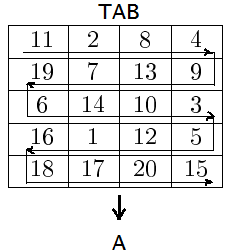
\includegraphics[scale=.6]{Allers-retours.png} 
\end{center}
 
 \vspace{-8mm}
\begin{center}
\begin{tabular}{|c|c|c|c|c|c|c|c|c|c|c|c|c|c|c|c|c|c|c|c|}
\hline 
 11 & 2 & 8 & 4 & 9 & 13 & 7 & 19 & 14 & 6 & 10 & 3 & 5 & 12 & 1 & 16 & 18 & 17 & 20 & 15 \\ 
\hline 
\end{tabular} 
  \end{center}
  %\textbf{  Attention : } il ne faut pas utiliser un autre  tableau interm�diaire 

\endinput
\solution
\begin{center}
\begin{minipage}{.7\textwidth}
 %footnotesize
  \lstinputlisting{Allers-retours.c}
%[firstline=1,lastline=10]
 \end{minipage}
 \end{center}